\documentclass[border=3pt]{standalone}
% Shared preamble for every generated figure.
% Matches the report: newtx (Times), greyscale, square boxes.
\usepackage{newtxtext,newtxmath}
% newtx's typewriter (txtt) draws a slashed zero; use Latin Modern instead.
\renewcommand{\ttdefault}{lmtt}
\usepackage{tikz}
\usetikzlibrary{positioning,arrows.meta,calc,fit,backgrounds,shapes.geometric,
                decorations.pathreplacing,decorations.pathmorphing,matrix,patterns}

\definecolor{figgrey}{gray}{0.88}
\definecolor{figmid}{gray}{0.60}
\definecolor{figdark}{gray}{0.35}

\tikzset{
  fig/.style={font=\small},
  box/.style={draw,thick,minimum height=8mm,minimum width=22mm,align=center,
              inner sep=2pt,font=\small},
  greybox/.style={box,fill=figgrey},
  smallbox/.style={draw,minimum height=6mm,minimum width=16mm,align=center,
                   inner sep=2pt,font=\scriptsize},
  ln/.style={-{Stealth[length=2.2mm,width=1.8mm]},thick},
  lnb/.style={{Stealth[length=2.2mm,width=1.8mm]}-{Stealth[length=2.2mm,width=1.8mm]},thick},
  lbl/.style={font=\scriptsize,inner sep=1.5pt},
  note/.style={font=\scriptsize\itshape,inner sep=1.5pt},
}

\begin{document}
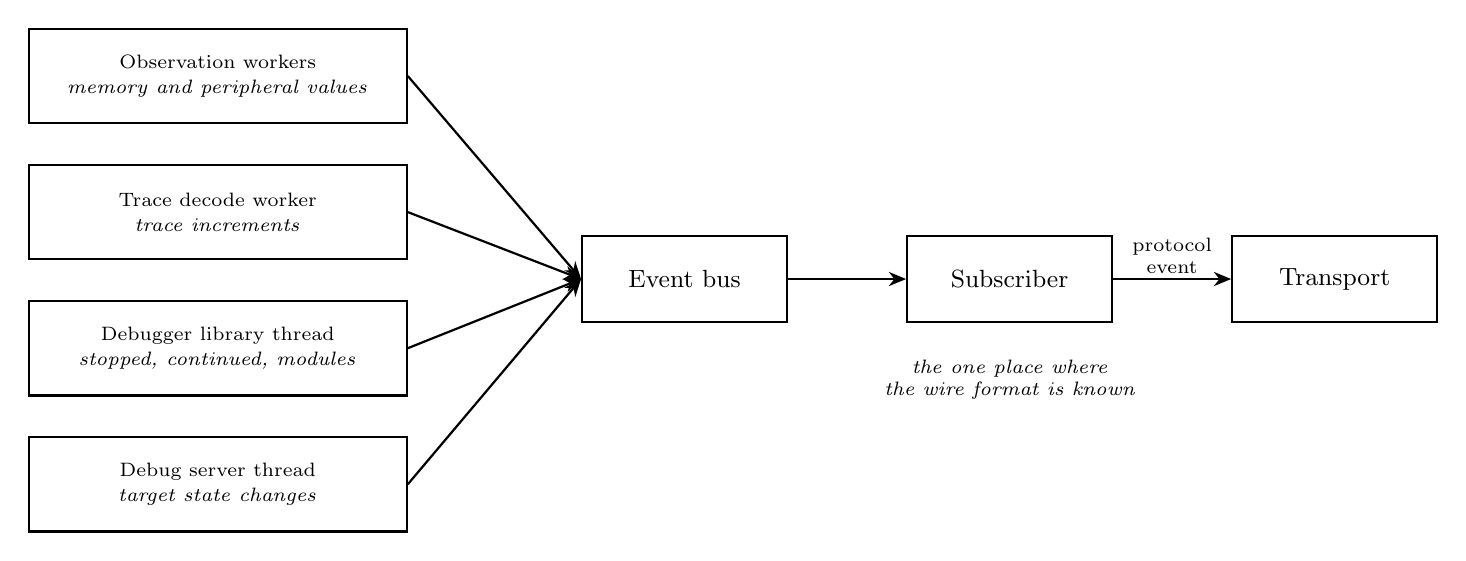
\begin{tikzpicture}[fig,
  pr/.style={draw,thick,minimum height=12mm,minimum width=48mm,align=center,font=\scriptsize},
  bx/.style={draw,thick,minimum height=11mm,minimum width=26mm,align=center,font=\small}]

\node[pr] (w1) {Observation workers\\[1pt]\textit{memory and peripheral values}};
\node[pr,below=5mm of w1] (w2) {Trace decode worker\\[1pt]\textit{trace increments}};
\node[pr,below=5mm of w2] (w3) {Debugger library thread\\[1pt]\textit{stopped, continued, modules}};
\node[pr,below=5mm of w3] (w4) {Debug server thread\\[1pt]\textit{target state changes}};

\node[bx,right=22mm of w2,yshift=-8.5mm] (bus) {Event bus};
\node[bx,right=15mm of bus] (sub) {Subscriber};
\node[bx,right=15mm of sub] (tx) {Transport};

\foreach \w in {w1,w2,w3,w4} \draw[ln] (\w.east) -- (bus.west);
\draw[ln] (bus) -- (sub);
\draw[ln] (sub) -- node[lbl,above,align=center]{protocol\\event} (tx);

\node[note,below=4mm of sub,align=center] {the one place where\\the wire format is known};

\end{tikzpicture}
\end{document}
